\chapter{Experiments}
\label{sec:experiments}

In this chapter the three Domain Adaptation Techniques \textbf{CycleGAN} \cite{DBLP:journals/corr/ZhuPIE17}, \textbf{CyCADA} \cite{DBLP:journals/corr/abs-1711-03213} and \textbf{SG-GAN} \cite{DBLP:journals/corr/abs-1801-01726} will be compared by analysing similarities and differences. Furthermore pretrained models of each architecture were used to generate translated images on which a pretrained DeepLabv3 \cite{DBLP:journals/corr/ChenPSA17} model then was used to perform semantic segmentation and the results will be compared on their Intersection over Union scores.

%\section{training the nets on tcml cluster} \todo{is this necessary or can we just use provided pre-trained models?}
%To train the models the tcml cluster of uni tübingen was used (\todo{add link to cluster website}). The cluster contains a lot of computing power with multiple compute nodes and a storage node. Each compute node has 4 CPUs and a NVidia 1080 Ti GPU and lots of RAM. In order to run the training code, it is necessary to create an .sbatch file. This file specifies how long a script needs to run, how much memory it needs and includes bash commands to run the script. Depending on what is specified in that .sbatch file the slurm manager system allocates ressources for that job and runs it as soon there are resources ready. While training cycleGAN mode collapse happened and the test images didn't get translated at all. Also to train for the 200 recommended epochs it would take around 2-3 weeks due to training taking a day for around 14 epochs. This is probably due to the fact that training cycleGAN is only possible on batches of size 1 which makes the vast resources available on the cluster not usable to their full potential. Also the student account can only run one job at once which makes it impossible to train different methods (cycleGAN, CyCADA, GradGAN) at the same time. Another issue is that it was not possible to visualize loss of generators and discriminators in order to supervise the training process and check if mode collapse or any other issue appeared. 

\section{Datasets}

\subsection{Synthetic dataset: \\
	Playing for Data: Ground Truth from Computer Games}

The GTA5 (Grand Theft Auto V) dataset is proposed in \cite{Richter_2016_ECCV}. It contains 24966 images taken from a street view in the game Grand Theft Auto V by Rockstar Games \cite{GTAV}. The images are provided with $1914 \times 1052$ pixels and are containing moving cars, objects, pedestrians, bikes, have changing lighting and weather conditions aswell as day and night scenes. For all of these images the authors provide ground-truth semantic label maps that are compatible with the classes of the Cityscapes dataset \cite{Cordts_2016_CVPR}. Detouring, i.e. injecting a wrapper between the game and the graphics hardware to log function calls and reconstruct the 3D scene is used to create the images. This also enables a faster labeling process as objects in a scene can be assigned an object ID through which assigned labels are propagated to other images containing this same object. Due to being more realistic than other existing synthetic street view datasets (e.g. SYNTHIA \cite{RosCVPR16}) the GTA5 dataset is very popular for training machine learning models related to autonomous driving and is therefore used in this work. Example images and corresponding label maps are shown in Figure \ref{fig:p4d_examples} 


\begin{figure}
	\centering
	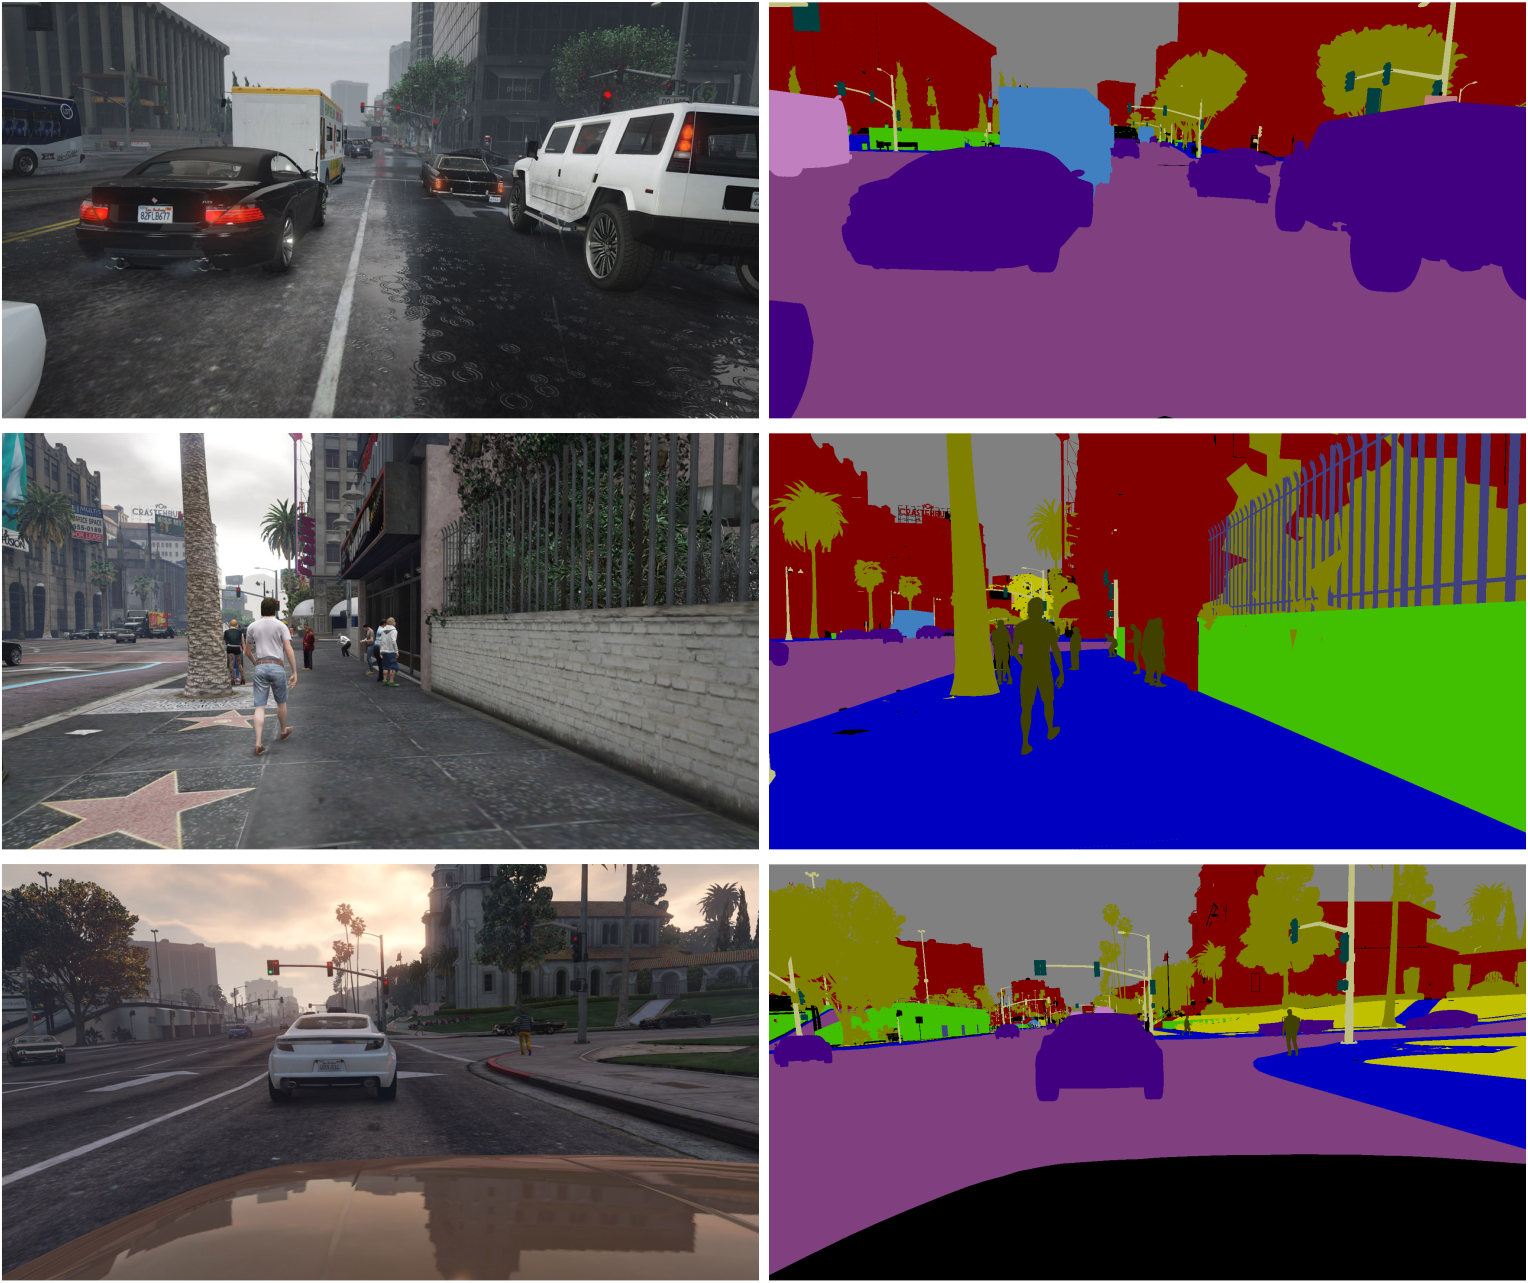
\includegraphics[width=\textwidth]{images/p4d_example.png}
	\caption{Example images (left) and corresponding ground-truth semantic label maps (right) provided in the GTA5 dataset \cite{Richter_2016_ECCV}.}
	\label{fig:p4d_examples}
\end{figure}

\subsection{Real dataset:\\
	The Cityscapes Dataset for Semantic Urban Scene Understanding}

The Cityscapes dataset \cite{Cordts_2016_CVPR} is a large scale dataset containing car dashcam view images from 50 european cities. It includes 30 classes relevant for autonomous driving. The images include scenes in spring, summer and fall seasons and under different weather conditions. There are 5000 images provided together with fine annotations and 20000 together with coarse annotations. Due to the large amount of labeled data from a dashcam view and the inclusion of scenes with different weather and lighting conditions this dataset is often used to train deep neural networks that are related to autonomous driving. Due to the popularity and the GTA5 dataset containing compatible label maps, this work uses Cityscapes as the real dataset for the experiments. See Figure \ref{fig:cityscapes_examples} for Example images.

\begin{figure}
	\centering
	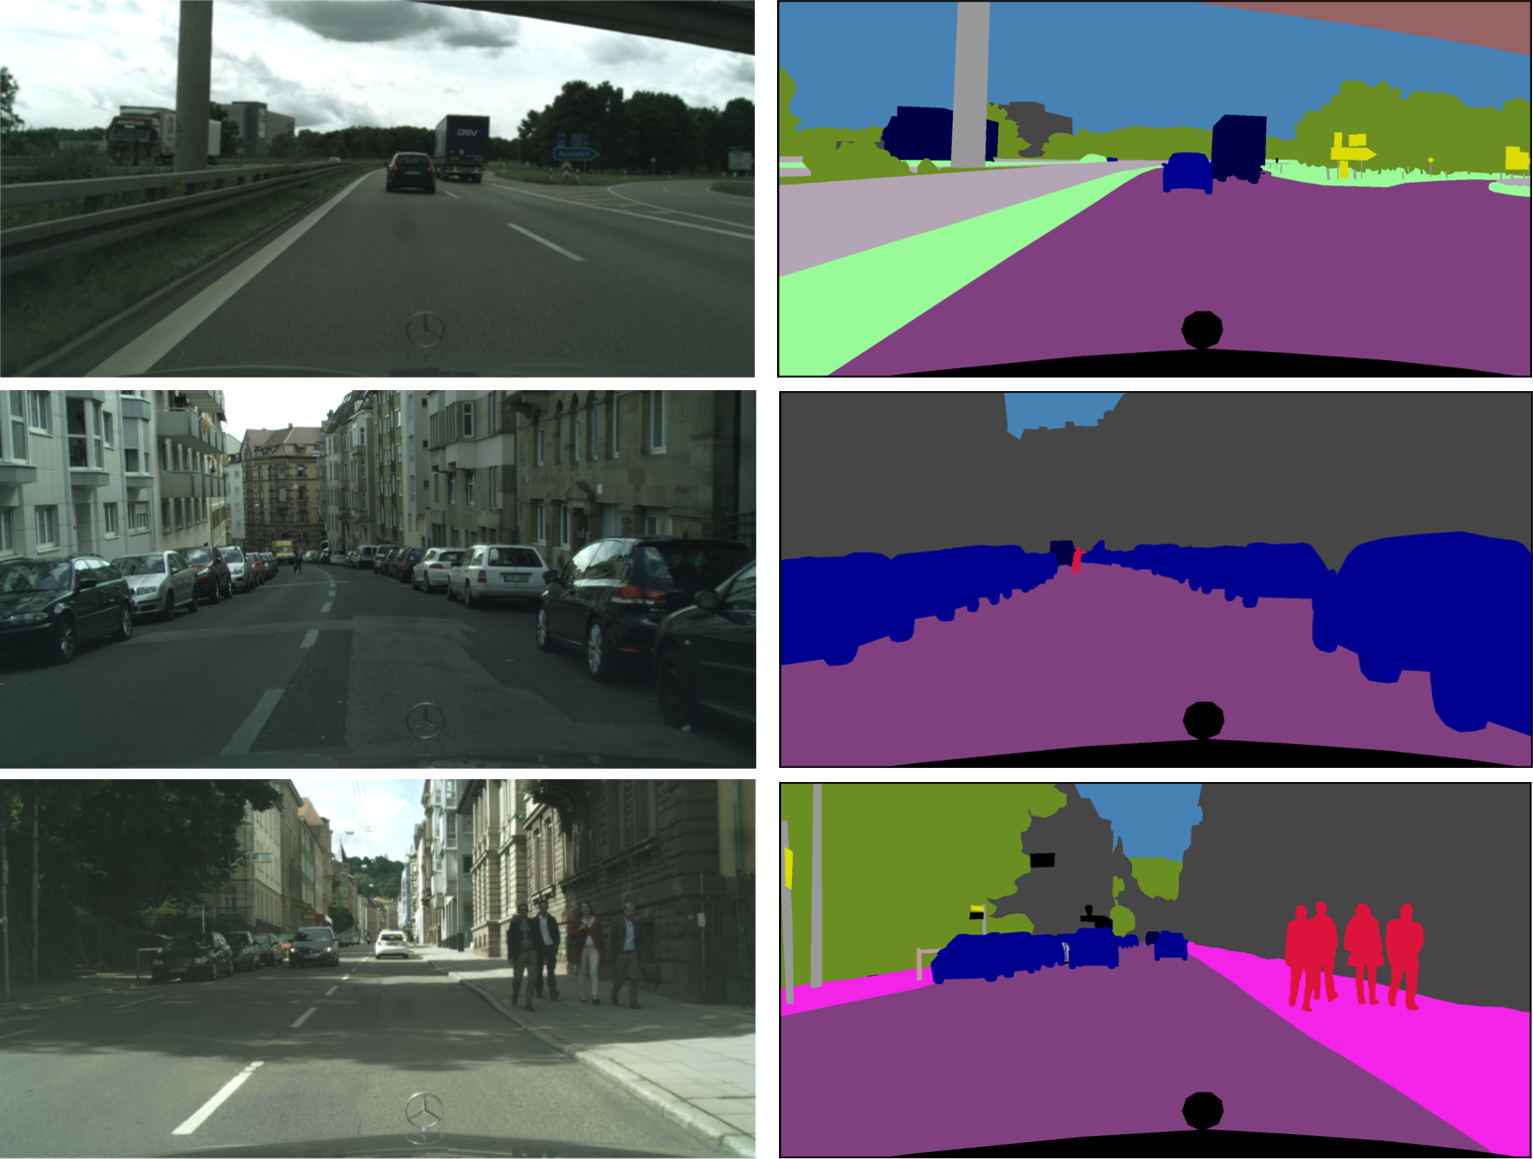
\includegraphics[width=\textwidth]{images/cityscapes_example.png}
	\caption{Example images (left) and corresponding ground-truth semantic label maps (right) provided in the Cityscapes dataset \cite{Cordts_2016_CVPR}.}
	\label{fig:cityscapes_examples}
\end{figure}

\section{Comparison Benchmark}
\subsection{Semantic Segmentation}
As this work is focused on datasets containing driving scenes the methods compared are applied to images that will then be performed semantic segmentation on. For the comparison Intersection over Union (IoU) is used. Intersection over Union is a metric often used to compare semantic segmentation methods' performance. All of the compared techniques were evaluated using IoU. It follows the following formula:
\begin{align*}
	\frac{\text{predicted pixels} \cap \text{ground truth pixels}}{\text{predicted pixels} \cup \text{ground truth pixels}}
\end{align*}
where predicted pixels are the pixels predicted for a specific class by the semantic segmentation model and ground truth pixels are the pixels containing the ground truth for that image. Usually there are multiple different classes to predict and therefore it is common to calculate the mean IoU (mIoU) over all images that have predictions. To compare how well classes themselves are predicted by a model, one can also calculate the class IoU (cIoU).

\section{Methodology}
For the comparison each technique was used to translate a sample of 500 images from the GTA dataset to the Cityscapes domain. For CycleGAN and SG-GAN each, the authors provided pre-trained models. For CyCADA pretranslated images are provided in the project repository \cite{CyCADA}. Due to CyCADA only providing 22k translated images instead of the full 25k images provided in the GTA dataset, from the randomly chosen 500 images only 450 are available here. This has to be regarded in the following comparison. To translate images with SG-GAN and CycleGAN the provided code \cite{SG},\cite{Cycle} and for the semantic segmentation task an implementation \cite{DLR} of deeplabv3 \cite{DBLP:journals/corr/ChenPSA17} was used. To compute the IoU values the deeplabv3 implementation uses the benchmark code provided by Cityscapes \cite{CSR}. All computations were run on Ubuntu 18.04 using CPU only in VirtualBox on a Windows Machine due to issues with dependencies while running the code on the tcml cluster of the university of tuebingen \cite{tcml}, a cluster for machine learning applications.

\section{Results}
The results are not as expected. As seen in Table \ref{table:results} semantic segmentation on CyCADA-translated images is just approximately 0.9 \% points more accurate than untranslated GTA images. SG-GAN is around 10 \% points less accurate than CyCADA and GTA5. Translating the images with SG-GAN worsened semantic segmentation results of the Deeplabv3 model. 
\begin{table}
	\centering
	\begin{tabular}{|c|c|c|c|}
		\multicolumn{4}{c}{\textbf{category Scores}}\\
		\hline
		\multicolumn{1}{c}{} & \multicolumn{3}{c}{Methods}\\
		\cline{2-4}
		\multicolumn{1}{c|}{category} & GTA5 & CyCADA & SG-GAN \\ 
		\hline
		construction & \textbf{0.740} & 0.719 & 0.651 \\ 
		\hline 
		flat & 0.709 & \textbf{0.894} & 0.639 \\ 
		\hline 
		human & \textbf{0.522} & 0.438 & 0.475 \\ 
		\hline 
		nature & 0.606 & \textbf{0.617} & 0.584 \\ 
		\hline 
		object & \textbf{0.100} & 0.077 & 0.085 \\ 
		\hline 
		sky & \textbf{0.894} & 0.841 & 0.518 \\ 
		\hline 
		vehicle & 0.661 & \textbf{0.694} & 0.641 \\ 
		\hline \hline
		average & 0.604 & \textbf{0.611} & 0.513\\
		\hline
		\multicolumn{4}{c}{}\\
		\multicolumn{4}{c}{\textbf{class Scores}}\\
		\hline
		\multicolumn{1}{c}{} & \multicolumn{3}{c}{Methods}\\
		\cline{2-4}
		\multicolumn{1}{c|}{class} & GTA5 & CyCADA & SG-GAN \\ 
		\hline
		bicycle & \textbf{0.127} & 0.055 & 0.062 \\ 
		\hline 
		building & \textbf{0.732} & 0.669 & 0.608 \\ 
		\hline 
		bus & 0.224 & \textbf{0.345} & 0.276 \\ 
		\hline 
		car & 0.652 & \textbf{0.665} & 0.620 \\ 
		\hline 
		fence & \textbf{0.201} & 0.186 & 0.169 \\ 
		\hline 
		motorcycle & 0.304 & 0.365 & \textbf{0.383} \\ 
		\hline 
		person & \textbf{0.501} & 0.419 & 0.455 \\ 
		\hline 
		pole & 0.0 & 0.0 & 0.0 \\ 
		\hline 
		rider & \textbf{0.460} & 0.314 & 0.366 \\ 
		\hline 
		road & 0.657 & \textbf{0.781} & 0.582 \\ 
		\hline 
		sidewalk & \textbf{0.370} & 0.314 & 0.315 \\ 
		\hline 
		sky & \textbf{0.894} & 0.841 & 0.518 \\ 
		\hline 
		terrain & \textbf{0.304} & 0.299 & 0.260 \\ 
		\hline 
		traffic light & \textbf{0.197} & 0.174 & 0.181 \\ 
		\hline 
		traffic sign & \textbf{0.156} & 0.108 & 0.143 \\ 
		\hline 
		train & 0.013 & 0.002 & \textbf{0.024} \\ 
		\hline 
		truck & 0.267 & \textbf{0.364} & 0.286 \\ 
		\hline 
		vegetation & 0.657 & 0.606 & \textbf{0.663} \\ 
		\hline 
		wall & 0.222 & \textbf{0.298} & 0.260 \\ 
		\hline \hline 
		average & \textbf{0.365} & 0.358 & 0.325\\
		\hline
	\end{tabular} 
	\caption{Intersection over Union results for evaluation on untranslated GTA5 images and translated images by CyCADA and SG-GAN respectively. Rounded to 3 decimal places}
	\label{table:results}
\end{table}

\subsection{Quantitative}

\subsection{Qualitative}

\section{Discussion}

